
This chapter is dedicated to the methodology that we propose to exert to achieve the objectives of this thesis, i.e. Methodology and Algorithms for High-level Modeling of Cosmic Radiations Impacts on Electrical Systems.



\section{Relation to State-of-the-Art}
Starting from the background, the facts established in the Chapter~\ref{intro}--- the digital circuits vulnerable to radiations require high-reliability requirements. The faults due to particle strikes cause different effects in the system behavior, e.g., stuck-at-fault. As discussed in~\ref{related} in digital sequential circuit, a single event upset cause a multiple faulty response of the underlying circuit. Consider an example of  a 3-bit counter as shown in Figure~\ref{fig:counter} the node is stuck-at-1$\rightarrow O_0$. This stuck node response can propagate to multiple outputs, as shown in Table~\ref{s@1-O0} and produce multiple erroneous outputs. The way this SEU interrupt at high-level of abstraction could typical manifest multiple correlated; "change in states of the design", and "change in signature values." To model the fault occur at the low level, and make the model of the faulty response of the circuit at high-level of abstraction, I propose to use the Hidden Markov Model. 



\begin{figure}[tb!]

 \centering
  \captionsetup{justification=centering}    
   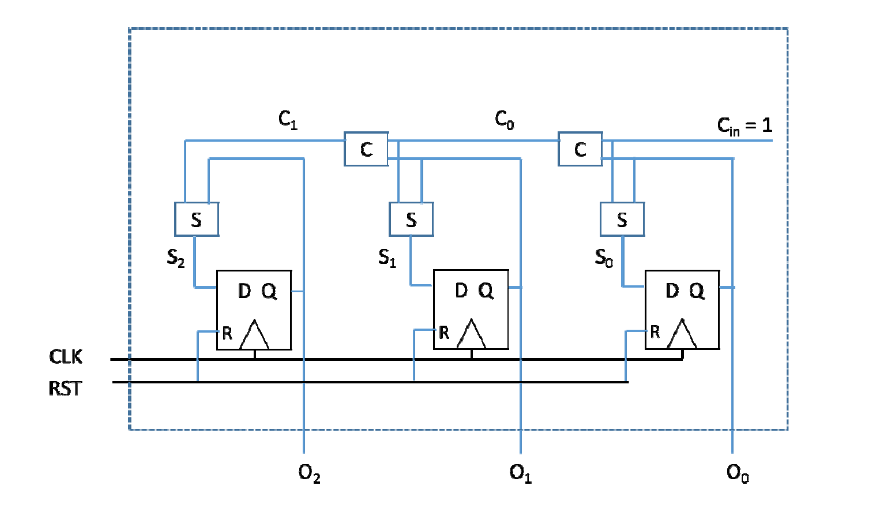
\includegraphics[scale=0.6]{Figures/counter.png}
   \caption{Signature Generation}
\label{fig:counter}
\end{figure}



\begin{table}[tb!]
\center
\caption{Stuck-at-1$\rightarrow O_0$}

\label{s@1-O0}

\begin{tabular}{|c | c| c | c| } 
 \hline
 \rowcolor{lightgray}
Faulty Value (Binary) & Faulty Value & Original Value & Arithmetic Signature   \\ 
\hline

 
 
 001& 1 &0 & -1  \\
 \hline
 011 & 3 & 1 & -2 \\ 
 \hline
 
 101 & 5 & 2 & -3 \\
 \hline
 111& 7& 3& -4 \\
 \hline
 001 & 1  &  4& 3 \\
 \hline
 011 & 3 & 5 &2  \\
 \hline
 101 & 5 & 6 & 1 \\
 \hline
 111 & 7 & 7 & 0 \\
 \hline
 
 
\end{tabular}
\end{table}




\section{Why Hidden Markov Model?}


We used the HMM for modeling and analysis of the sequential circuits susceptible to soft-errors. We prefer to use the HMM analysis over the other modeling techniques, e.g., BDD/ADD, Boolean Satisfiability problem (SAT), Monte-Carlo sampling, approximate approaches, symbolic methods for efficient estimation, simulator methods. As all these techniques require to transform the circuit into their respective tool and require a lot of mathematical notations. While in HMM we can directly make the model just looking into the signature values, construct the high-level model that can be further use for the analysis. The HMM can be used very well to model systems which consists of different observable outputs on different hidden conditions.

To make the HMM. Firstly, we need to have two copies of the original circuit --- named Fault-Free circuit, and a Faulty circuit (\textit{hit circuit}). The Fault free circuit is used to collect the correct behavior of the circuit (fault-free outputs), and faulty is used to collect the faulty response of the circuit (faulty output). The difference between them give us the signature as shown in the Figure~\ref{fig:SG} and depicted in the following equation.

\begin{center}
$Arithmetic$ $Signature$ $=$ $Original$ $Value$ $-$ $Faulty$ $Value$
\end{center}



 \begin{figure}[tb!]

 \centering
  \captionsetup{justification=centering}    
   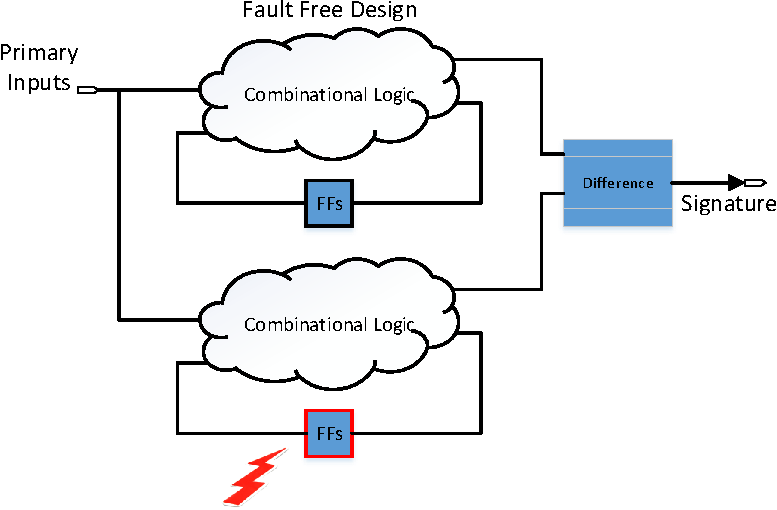
\includegraphics[scale=0.8]{Figures/signature1.pdf}
   \caption{Signature Generation}
\label{fig:SG}
\end{figure}




Hidden Markov Model is a statistical model in which a system can be modeled is assumed to be a Markov process with unobserved, i.e., hidden states. A Markov process  is a stochastic process that satisfies the Markov property -- \underline{memorylessness}, meaning, a process that satisfies the Markov property if the prediction of the future of the system output based solely on its present state, it is independent of the future and past states. Inorder to apply the HMM, we need a system that generate probabilistic output patterns in time, e.g., faulty response of the 3-bit counter, as a result the node is stuck-at-fault. Afterwards, we need to look at the system and need to know which state of the system give that particular output ---  the underlying system is hidden. For example, in the case of a three bit counter, the observed sequence is the "signature" and the hidden is the "stuck-at-node." Now, we wish to devise a model to predict "stuck-at-node", without actually knowing about the node. It is important to note that the number of states in the hidden process and the number of observable states may be different. 


In the 3-bit counter example, there are total n-nodes where the signal can get stuck (stuck-at-1, and stuck-at-0) both are possible. and we can get the  different signatures (chapter Preliminaries derive signatures for all the nodes). Here for simplicity, I can give the example of four different signatures and construct the HMM. The signarures are: \textit{Sign-1, Sign-2, Sign-3, and Sign-4}. The observed signatures are probabilistically related to the hidden process. We can model such process using a hidden Markov model, where there is an underlying hidden Markov process changing over time, and a set of observable states which are related to somehow to the hidden states.


The figure~\ref{fig:HMM-3-bit} shows the Markov model for the hidden and the observable states for the 3-bit counter example. The hidden states are (stuck-at-nodes), and observable states are  the signatures. 


\begin{figure}[tb!]

 \centering
  \captionsetup{justification=centering}    
   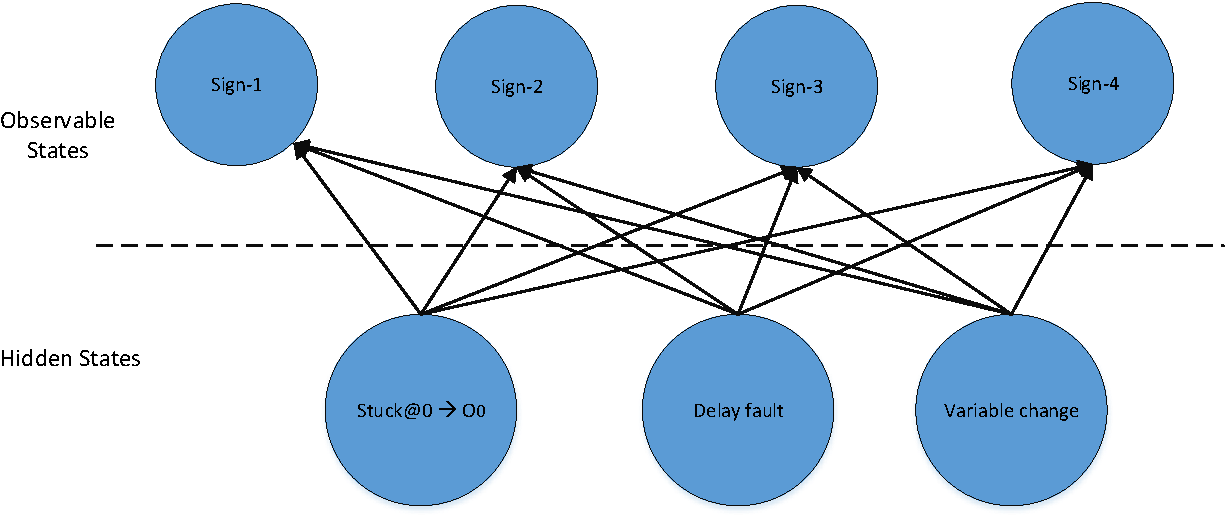
\includegraphics[scale=0.8]{Figures/HMM.pdf}
   \caption{HMM model 3-bit counter.}
\label{fig:HMM-3-bit}
\end{figure}




The HMM is based on  the two things:a) Observable States, and b) Hidden States. If we closely observe above mentioned 3-bit counter example, we realized that in that scenario --  signatures are the observable state, and the fault occur due to the bit-flip that cause some node in the circuit to stuck, i.e., stuck-at-1 $\rightarrow$ $O_o$ is the hidden state. In this thesis, we used the concept of HMM to construct the high-level model based on the signature information.





\section{Modeling Hidden Markov Model}


\begin{figure}[tb!]

 \centering
  \captionsetup{justification=centering}    
   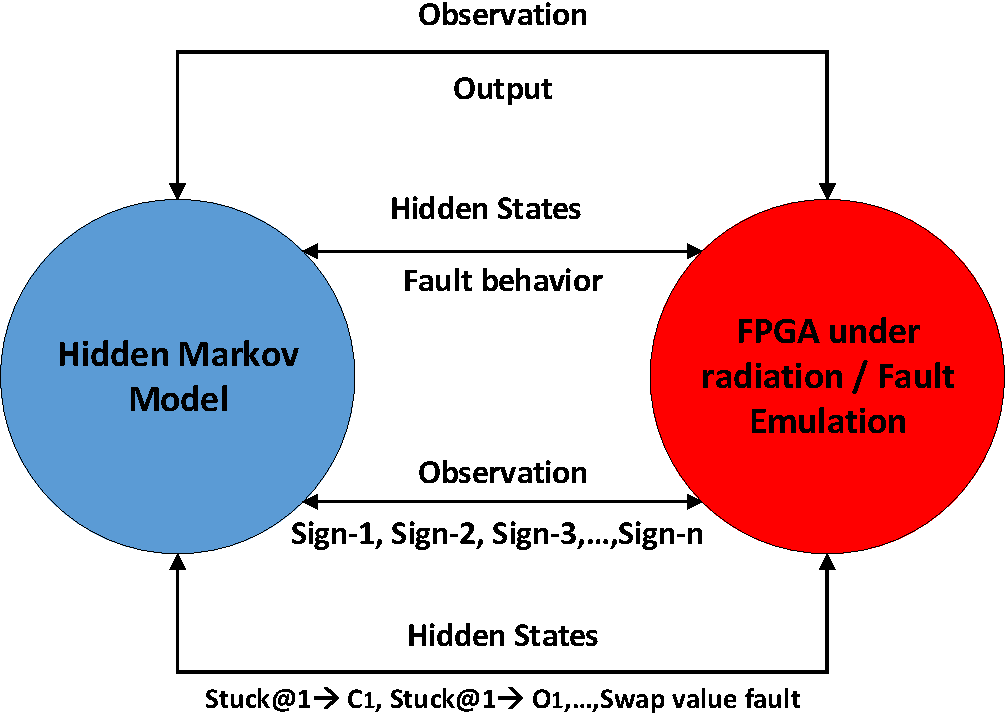
\includegraphics[scale=0.8]{Figures/HMM-air.pdf}
   \caption{Hidden Markov Model to the FPGA based fault emulation system}
\label{fig:HMM-air}
\end{figure}


The Figure~\ref{fig:HMM-air} shows the basic HMM applied to the FPGA based fault emulation system. We model this system with the HMM, where, the outputs emitted by the system (FPGA under radiation/ Fault Emulation) are observable (signatures --- in our problem domain), not underlying states of the system (Stuck-at-fault). The HMM can be visualized as a simple finite state machine. The HMM has a strong statistical foundation; it has the ability for efficient learning algorithm, which can take place directly from the raw sequence data. \textbf{The problem in hand:} can be solved by using the HMM as we can observe the sequence of signatures, but we do not know the which states (stuck-at-node) of the system went through to generate that particular signature. The analyses of Hidden Markov Model seek to recover the states from the observed data.








\subsection{Probabilities in a HMM}

There are three important things to know about the probabilities in HMM.

\begin{itemize}
\item The connections between the hidden states of the system, and the observable states of the system represent the probability of generating a particular observed state given that the Markov process is in a particular hidden state.

\item The probabilities entering into the observable states will sum to "1." 

\begin{center}
$Pr(Sign-1|Stuck) + Pr(Sign-1|Stuck) + Pr(Sign-1|Stuck)  = 1 $
\end{center}

\item In addition, probabilities define the Markov process, we have another matrix termed as "confusion matrix", which contains the probabilities of the observable states given a particular hidden state. The following matrix is the confusion matrix for the 3-bit counter example.


\begin{center}


CM = \bordermatrix{~& Sign-1 & Sign-2 & Sign-3 & Sign-4\cr
                  Stuck@1\rightarrow{C_0}& 0.60 & 0.20 & 0.15&0.05 \cr
                  Stuck@1\rightarrow{C_1} & 0.25 & 0.25 &0.25 &0.25\cr
                  Stuck@1\rightarrow{O_0} & 0.05 & 0.10 &0.35 &0.50\cr}
\end{center}
\end{itemize}


\subsection{HMM Parameters}

A hidden Markov Model is described as $(\Pi, A, B)$ as shown in Figure~\ref{MARKOV-SERIS}, Where,


\begin{figure}[tb!]

 \centering
  \captionsetup{justification=centering}    
   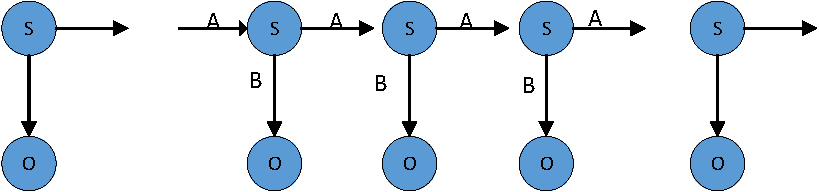
\includegraphics[scale=0.8]{Figures/MARKOV-SERIS.pdf}
   \caption{HMM Formalization.}
\label{fig:MARKOV-SERIS}
\end{figure}


\textbf{$\Pi = (\pi_i)$ initial state probabilities vector;}




$A = (a_ij)$ state transistion matrix;  \hspace{0.3cm} $P_r(x_i | {x_j}_{t-1})$

$B = (b_ij)$ confusion matrix;     \hspace{0.3cm}        $P_r(y_i | x_j)$


We can find the initial state probability vector,state transistion matrix and confusion matrix  from our experimental data generated by the radiation or emulation experiment.

\textbf{Hidden States:} The true states of the system that may be described by a Markov Process, e.g., Stuck-at-fault, some particular node.

\textbf{Observable State:} The state of the process, visible, e.g., Signature.
\textbf{$\Pi$ $Vector$:} contains the probability of the hidden model being in a particular hidden state (stuck-at-node) at time t = 1.

\textbf{state transition matrix:}  holding the probability of a hidden state given the previous hidden state.

\textbf{confusion matrix:} containing the probability of observing a particular observable state given that the hidden model is in a particular hidden state. 



Once we model a system with HMM, it helps to find three problems. We model them according to our problem, i.e.,

\begin{tcolorbox}[width=\textwidth,colback={gray},title={Evaluation },colbacktitle=gray,coltitle=black]  

Find the probability of an observed signature given a HMM.  
\end{tcolorbox}


\begin{tcolorbox}[width=\textwidth,colback={gray},title={Decoding },colbacktitle=gray,coltitle=black]  

Finding the hidden states (stuck-at-fault) that most probably generated an observed sequence. 
\end{tcolorbox}

\begin{tcolorbox}[width=\textwidth,colback={gray},title={Learning },colbacktitle=gray,coltitle=black]  

The third problem is generating an optimized HMM given a sequence of signatures (observations).
\end{tcolorbox}



\section{HMM Application for Signature}

Hidden Markov Model can give the answer of three major questions that we can use in our problem domain. It helps to a) compute the probability of a given sequence of signatures, b) compute the most probable sequence of states, and c) given a sequence of observations and learn the best HMM model.

In order to find the solution of these three questions, we called it HMM applications.


\textbf{The Three basic HMM Applications}

\begin{itemize}
\item Applications 1 : Probability Evaluation
 \begin{itemize}
 \item How do we efficiently compute the (probability of the signatures given that the HMM parameters) $P(O|\Pi)$ from the given observed signature sequence $O = {O_1, O_2,...,O_n}$.
 
  \begin{itemize}
  \item We can use the forward algorithm~\cite{ghahramani1996factorial}.
  \end{itemize}
 \end{itemize}
\end{itemize}

\begin{itemize}
\item Application 2 : Optimal State Sequence
 \begin{itemize}
 \item Given signatures sequence $O = {O_1, O_2,....,}O_n$ and model $\Pi$ how do we choose a hidden state sequence (stuck-at-fault) $Q={q_1,q_2,q_3,...q_n}$
that is optimal, i.e., best explains the data. 
  \begin{itemize}
  \item The Viterbi algorithm~\ref{forney1973viterbi} helps to find the answer of this application
  \end{itemize}
 \end{itemize}
\end{itemize}



\begin{itemize}
\item Application 3 : How do we adjust the parameters of the model $\Pi = {\pi, A, B}$ to maximize the likelihood $P(O|\pi)$ 
 \begin{itemize}
 \item Given observation sequence $O = {O_1, O_2,....,}O_n$ and model $\Pi$ how do we choose a hidden state sequence $Q={q_1,q_2,q_3,...q_n}$
that is optimal, i.e., best explains the data. 
  \begin{itemize}
  \item The solution is either to use Expectation-Maximization~\ref{moon1996expectation} or Baum-Welch re-estimation~\ref{leggetter1995maximum}.
  \end{itemize}
 \end{itemize}
\end{itemize}









\subsection{Evaluation Application}

For probability evaluation, we need to compute the likelihood of an observed signature sequence $O = {O_1, O_2,...,O_t}$ given a particular HMM model $ \Pi = {A, B, \pi}$. The computation of this probability involves all the possible hidden state sequence and evaluate the corresponding probability. 

\begin{itemize}

\item  $P(O | \Pi) = \sum\limits_{\forall Q}^{} P (O | X, \Pi) P (X, \pi)$ 

\item For a specific state sequence $X = {x_1, x_2,...,x_t}, P(O | Q, \Pi):$

 \hspace {0.2cm} $P (O | X, \Pi) = \prod_{t=1}^{T} P (o_t | q_t, \Pi) = \prod_{t=1^{T} b_{x_t} (o_t)}$
 
 \item The probability of the state sequence $X$:
 \\
 \hspace {0.2cm} $ P (X | \Pi ) = \pi_{x_1} a_{x_1 x_2} a_{x_2 x_3},...,a_{x_{T-1} x_T}$
 
 \item The final expression we get:
 


$P (O | \Pi ) = \sum\limits_{x_1, x_2,..., x_T} \pi_{x_1} b_{x_1} (o_{x_1}) a_{x_1 x_2} b_{q_2} (o_{x_2}),..., a_{x_{T-1} x_T} b_{xT} (o_{xT})$

\item If there are $N^T$ possible state sequence, this approach becomes infeasible to apply or implement even for the smaller circuits.

\begin{itemize}
\item For N = 5 and T = 100, the order of magnitude --- $10^7$
\end{itemize}
 

\end{itemize}

This problem can be solved by using the Forward Algorithm:

\textbf{Example:} Consider an example where we have a number of HMMs (a set of triplet $(\pi, A, B)$) describing different systems, and a sequence of observation, i.e., you will get these system by performing radiation/fault emulation experiments for hours of testing. You have number of HMMs constructed in the Simulink library and want to know which HMM most probably generated the given sequence (signature).


We will use the forward algorithm to calculate the probability of an observation sequence given a particular hidden Markov Model, and find the most probable HMM. Suppose that you have a HMM that describe the stuck-at-node, and we also have a sequence of signatures. Suppose the stuck-at-nodes works in this order $(stuck-at-c_0)$, $(stuck-at-c_1)$, $(stuck-at-O_1)$, the signatures: Sign-1, Sign-2, and Sign-3. There is some hidden relationship between stuck-at-node and the signatures, we can make a "Trellis" diagram as shown in Figure~\ref{fig:trellis}



\begin{figure}[tb!]

 \centering
  \captionsetup{justification=centering}    
   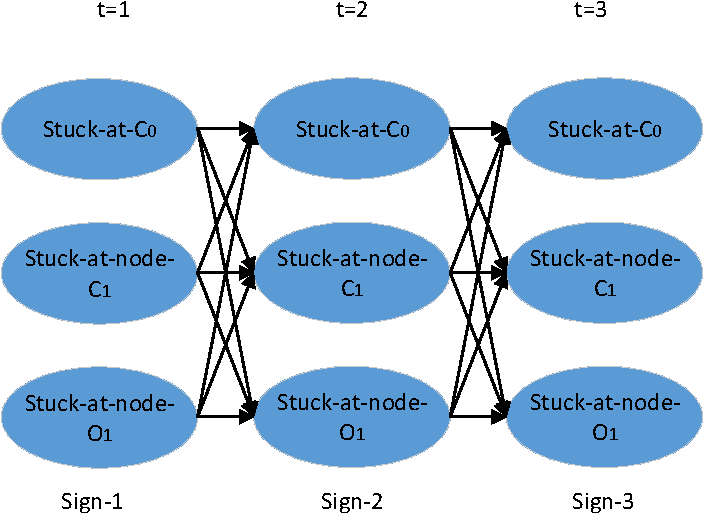
\includegraphics[scale=0.8]{Figures/trellis.pdf}
   \caption{Trellis Diagram}
\label{fig:trellis}
\end{figure}


From trellis figure we conclude the following:

\begin{itemize}

\item Each column in the trellis represents the possible state of the stuck-at-node and each state in column is connected to the each state in the adjacent column.

\item The transition between the states --- state transitions has the probability provided by the "state transition matrix."

\item Each column in the signature observations at that time: the probability of this signature observation given anyone of the above stuck-at-node state is provided by the confusion matrix. 

\item As mentioned above one of the possibility of calculating the probabilities of the observed states would be find each possible sequence of the hidden stuck-at-node states and sum all these probabilities. Just for this example, there would be $3^3 = 27$ possible sequences, its extremely complex to do this. So, we will propose to use the forward algorithm that can calculate the probabilities of observing a sequence recursively given a HMM.

\end{itemize}

\textbf{Forward algorithm Steps:}

We need to calculate the probability of observing a signature recursively given a HMM. 

\begin{enumerate}

\item The first step is the initialization step at t = 1 when there is no path to the state. The probability of being at state at t = 1 is actually the initial probability:
\begin{itemize}


 \item $P (state | t = 1) = \pi $
\item The initial probability at t = 1 is the probability multiplied by the associated observation probability.
$\alpha(j) = \pi(j) b_i (O_1)$
\end{itemize}

\item Second, we need to define a \textbf{partial probability} which is the probability of reaching an intermediate state in the trellis.

\begin{itemize}

\item For example, the T-long signature sequence: $(Y_k1, Y_k2,..., Y_kT)$, the partial probabilities $\alpha 's$. Figure shows the Trellis diagram. Calculate the probability of reaching an intermediate state in the trellis diagram as the sum of all possible paths to that state.

\item The partial probability of state $j$ at time $t$ is $t(j)$, to calculate the partial probability:

$\alpha_t(j) = P (observation | hidden state is j) \times P (all paths to state j at time t)$

\item The partial probabilities for the final observation hold the probability of reaching those states going through all the possible paths. The sum of these final partial probabilities is the sum of all possible paths. 

\hspace {4.5 cm}$\alpha_{t+1}(j) = b_jk_{t+1} \sum\limits^{n}_{i = 1} \alpha_t(i) a_{ij}$




\end{itemize}
\item This expression can be used to calculate the $\alpha$. We can find the probability of an observation given HMM. The probability of the sequence given the HMM is then the sum of the partial probabilities at time t = T. This is called termination step.
 
 \hspace {4.5 cm}$P(Y^K) = \sum\limits^{n}_{j=1} \alpha_T (j)$

\end{enumerate}







\subsection{Decoding Application}


\begin{figure}[tb!]

 \centering
  \captionsetup{justification=centering}    
   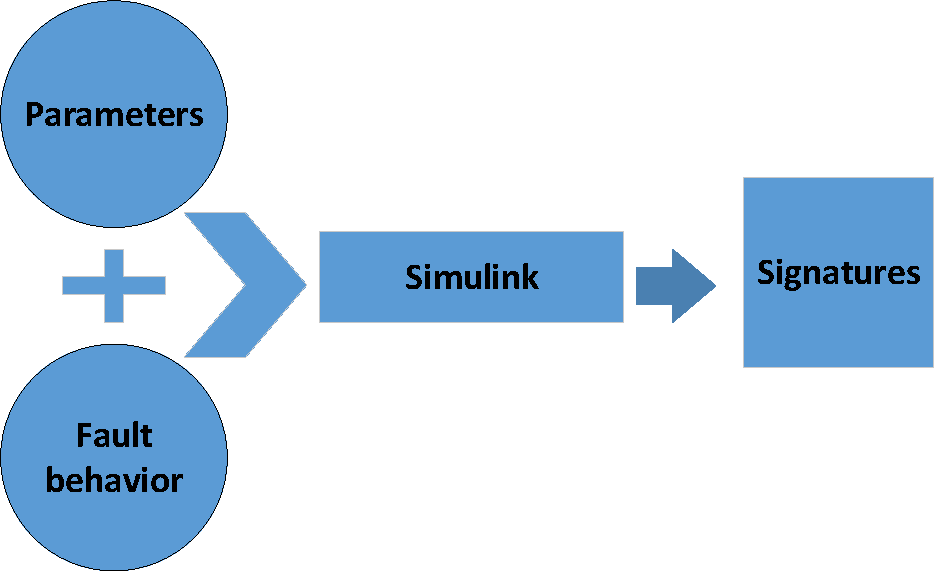
\includegraphics[scale=0.8]{Figures/fromhiddentosignature.pdf}
   \caption{Hidden states to Signatures}
\label{fig:HMMsig}
\end{figure}


To design it for the decoding application there are two possibilities to use either viterbi decoding algorithm or posterior decoding. The viterbi gives the most likely sequence while posterior decoding gives the most likely state at each position. Here, we are more focused on the sequence of hidden states (use in simulator to reproduce the signatures) that give the respective signatures, in this case viterbi algorithm is preferable. The decoding capability of HMM helps to find the sequence of the stuck-at-node that generated the given signatures. In the FPGA fault emulation and radiation experiment we are interested to find the stuck-at-fault nodes of the system as they represent some valuable information that can later be used to give to the Simulink model to reproduce the signatures (if we know the stuck-at-nodes and their respective probabilities) as shown in Figure~\ref{fig:HMMsig}.




 
\textbf{Example:} Consider an example of the signature and stuck-at-fault; an FPGA test designer can only sense the signature but wants to know the stuck-at-fault nodes to make the high-level model based on this information, i.e., hidden state. 

\textbf{Answer}: We will use the \underline{Viterbi Algorithm} to determine the most probable sequence of stuck-at-fault node by giving the sequence of signatures and HMM. Inshort, decoding helps to find the hidden sequence most likely to have generated a sequence of observation --- solved using Viterbi algorithm as shown in Figure~\ref{fig:HMMsig-Vit}.


\begin{figure}[tb!]

 \centering
  \captionsetup{justification=centering}    
   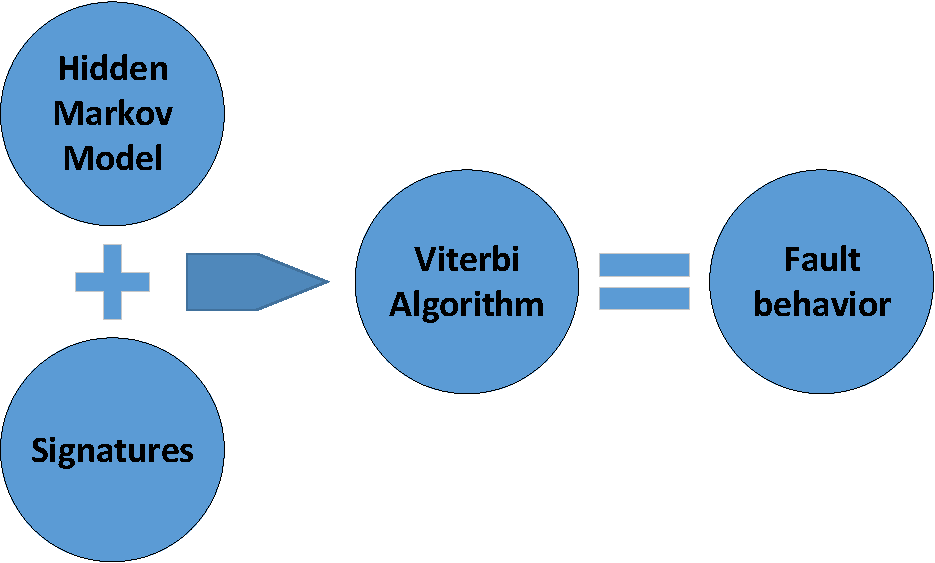
\includegraphics[scale=0.8]{Figures/HMM-plus-viterbi.pdf}
   \caption{Signatures to hidden states}
\label{fig:HMMsig-Vit}
\end{figure}

\subsubsection{Viterbi Algorithm}


The Viterbi algorithm is based on the assumption that the most \textit{likely} path (hidden states sequence), $Q^* = argmax_Q P(Q|O) $, is a good estimation of the sequence of hidden states that generated the observed sequence $(O)$. The viterbi algorithm generates a path $X = (x_1, x_2,...,x_T)$, which is a sequence of states $x_n \in S = {s_1, s_2,...,s_k}$ that produce the sequence of observations $Y = (y_1,y_2,...,y_T) \in {1,2,...,N}^T N$ $=$ $Observation$ $space$.

\textbf{Initialization:}



\begin{itemize}


\item The Observation space $O =  {o_1,o_2,...,o_N}$

\item the state space $S = {s_1,s_2,...,s_K}$

\item an array of the initial probabilities $\Pi = (\pi_1, \pi_2,...,\pi_K)$; $\pi_i is the probability the x_1 == s_i$

\item a sequence of observations $Y = (y_1,y_2,...,y_T)$; $yt == i$ the observation at time $t$ is $o_i$

\item the state transition matrix $A_ij$ stores the transition probability from state $s_i$ to $s_j$


\item emission matrix $B_ij$ stores the probability of observing $o_j$ from the state $s_i$
\end{itemize}  

\textbf{Recursion:}

We need to determine the hidden states by calculating $P(X|O)$. However, this brute force approach becomes intractable if the number of states gets larger, as the number of state path grows exponentially $(N^T)$. So, we need to calculate the $argmax_X P(X|O)$ . The most likely sequence is given by the recursion relations.

\begin{center}

\begin{itemize}


\item $V_1,k = P (y_1|k) \times \pi_k$

\item $V_t,k = max_{x \in S} (P (y_t|k) \times a_x,k \times V_t-1,x)$

\item $V_t,k$ probability of the most probably sequence $P (x_1, x_2,...,x_T, y_1,y_2,...,y_T)$

\end{itemize}

\end{center}


\textbf{Final:}

The most likely hidden state sequence $X = (x_1,x_2,...,x_N)$ 

%\textbf{Example}
%
%
%Consider you have an FPGA board, with some benchmark, e.g., counter is running on it. You need to  ask to perform a radiation induced experiment on it, derive the signatures, and make the high level model of it.
%
%Suppose at any given time, the system can be in one of N possible states.
%
%\begin{center}
%$S = {S_1, S_2,....., S_N}$
%\end{center}
%
%Consider you observed there are only three possible states in which system can go, e.g., stuck-at-1$\rightarrow O_{0}$, stuck-at-0$\rightarrow O_{1}$, and stuck-at-1$\rightarrow C_{1}$. Further observed that the transition between these states can be described by the transition matrix.
%
%
%\begin{center}
%
%
%A = {$a_ij$} = \bordermatrix{~& & & \cr
%                   & 0.4 & 0.3 & 0.3 \cr
%                   & 0.2 & 0.6 &0.2 \cr
%                   & 0.1 & 0.1 &0.8 \cr}
%\end{center}
%
%--- Question
%
%\begin{itemize}
%\item I model this behavior of the system in MATLAB and ask the high-level simulink designer you can find the response of the system as you like. He set the system paramters to know the faulty response of the system for the next seven different radiation experiment in order of (stuck-at-1$\rightarrow C_{1}$, stuck-at-1$\rightarrow C_{1}$, stuck-at-1$\rightarrow O_{0}$, stuck-at-1$\rightarrow O_{0}$, stuck-at-1$\rightarrow C_{1}$, stuck-at-0$\rightarrow O_{1}$, stuck-at-1$\rightarrow C_{1}$  ) given that the outcome of first radiation experiment is stuck-at-1$\rightarrow C_{1}$.
%
%\item \textbf{Answer}
%
%
%\item P(stuck-at-1$\rightarrow C_{1}$, stuck-at-1$\rightarrow C_{1}$, stuck-at-1$\rightarrow O_{0}$, stuck-at-1$\rightarrow O_{0}$, stuck-at-1$\rightarrow C_{1}$, stuck-at-0$\rightarrow O_{1}$, stuck-at-1$\rightarrow C_{1}$ | model)
%\end{itemize}
%
%\hspace{0.2cm} = P(stuck-at-1$\rightarrow C_{1}$) P(stuck-at-1$\rightarrow C_{1}$| stuck-at-1$\rightarrow C_{1}$) P(stuck-at-1$\rightarrow C_{1}$| stuck-at-1$\rightarrow C_{1}$) P(stuck-at-1$\rightarrow O_{0}$|stuck-at-1$\rightarrow C_{1}$) P(stuck-at-1$\rightarrow O_{0}$|stuck-at-1$\rightarrow O_{0}$) P(stuck-at-1$\rightarrow C_{1}$|stuck-at-1$\rightarrow O_{0}$) P(stuck-at-0$\rightarrow O_{1}$|stuck-at-1$\rightarrow C_{1}$) P(stuck-at-1$\rightarrow C_{1}$| stuck-at-0$\rightarrow O_{1}$)
%
%\hspace{0.2cm} = $\pi_3$ $\times$ $a_33$ $\times$ $a_33$ $\times$ $a_13$ $\times$ $a_11$ $\times$ $a_31$ $\times$ $a_23$ $\times$ $a_32$
%
%\hspace{0.2cm} = $1 \times 0.8 \times 0.8 \times 0.1 \times 0.4 \times 0.3 \times 0.1 \times 0.2$
%
%The above mentioned model assumes that each state can be uniquely associated with an observable event. This model is too restrictive to be used for most of the realistic problems like ours, where we have no information of the underlying system only observe the outcome due to the result of change in hidden state.

\subsection{Learning}

The third application of the HMM is optimizing the parameters of the model. There are two possible solutions of this problem either to chose supervised learning and unsupervised learning.  In supervised learning you have one input variable, one output variable and use the algorithm to learn the mapping from the input to output, e.g., logistic regression, linear regression. We can map our problem to supervised learning, our goal is find the mapping function that when we have a new signature the mapping function can predict the stuck-at-node. Now, consider a case where I have only signature data and no information how these signatures comes from stuck-at-nodes.  This is the unsupervised learning because there is no answer available. In this thesis problem we opt for the unsupervised learning, because we have only the data available is signature, and we will find the parameters that maximize the probability of the hidden sequence.  

We can also find the optimal solution for our model by using the learning application of the HMM. The learning application works on the model parameters and observations to find the model that fits the data. There are three different techniques to do: a) Maximum Likelihood Estimation, b) Viterbi Training, and c) Baum  Welch = Forward-Backward Algorithm. 


Suppose we have a HMM: $\Pi = (\pi, A, B)$. The Baum-Welch algorithm is used to find  a local maximum for $\Pi^* = arg max_{\Pi} P (O | \Pi)$, i.e., the HMM parameters $\Pi$ that maximize the probability of the observation.

The Baum-Welch works in the following way:

\begin{enumerate}


\item Find the forward probabilities with the forward algorithm.


\begin{itemize}
\item $\alpha_{i}(1) = \pi_{i} b_{i} (o_{1})$
\item $\alpha_{i}(t + 1) = b_{i}(o_{t+1}) \sum\limits^{N}_{j=1}\alpha_{j}(t)a_{ji}$

\end{itemize}

\item Find the backward probabilities with the backward algorithm.

\begin{itemize}
\item $\beta(t) = P(o_{t+1} o_{t+2},...,o_{T} | x_{t} = i, \Pi) $

\item $\beta_{i}(T) = 1$
\item $\beta_{i}(t) = \sum\limits^{N}_{j=1} a[x_i, x_j] b[x_j,o_{t + 1}\beta_{j}(t + 1)]$

\end{itemize}
\item Find the probability of state $i$ at time $t$

\begin{itemize}

\item $P (x_t = i, O | \Pi) = P (o_1, o_2,...,o_t, x_t = i | \Pi) P (o_{t + 1}, o_{t + 2},...,o_{T} | x_{t} = i, \Pi) == \alpha_{i}(t) \beta_{i}(t) $

\item use the Bayes Theorem:

$P(x_t = i | O, \Pi) = \frac{P(x_t = i, O | \Pi)}{P(O | \Pi)} = \Upsilon_{i}(t)$

\end{itemize}
\item Find the probability of a transition from state $i$ to state $j$ at time $t$

\begin{itemize}
\item $\xi_{t}(i,j) = P (x_t = i,x_{t + 1} = j | O, \Pi)$


\item These probabilities can be computed bu using the forward and backward variables:

$\xi_{t}(i,j) = \frac{\alpha_i (t) a[x_i x_j] b[x_j,o_{t + 1}] \beta_j (t + 1)   }{P(O | \Pi)}$

\end{itemize}
\item Find the expected transition and emission counts:

$\sum\limits_{t = 1}^{ T } \Upsilon_i (t)$ = expected number of transition from $x_i$

$\sum\limits_{t = 1}^{ T} \xi_t (i ,j)$ = expected number of transition from $x_i$ to $x_j$

\item Perform the parameter estimation by the ratio of expected count the maximization step:


$\overline{a}[x_i, x_j] = \frac{\sum\limits_{t = 1}^{T - 1}\xi_{t} (i, j)}{\sum\limits_{t = 1} T - 1 \Upsilon_{j}(t)} $




$\overline{b}[x_i, o_k] = \frac{\sum\limits_{t = 1}^{T - 1}\Upsilon_{j} (t) 1 (o_t = k)}{\sum\limits_{t = 1}^{T - 1} \Upsilon_{j}(t)} $

\item Stop the computation when the change in the log likelihood is smaller than a given threshold or the maximum iterations are passed.

\end{enumerate} 















\section{Utilization}



Once we have all the information as shown in Figure~\ref{fig:lib} about the stuck-at-fault nodes, signatures, HMM parameters, probabilities of the stuck-at-node. We can create the libraries of the faulty components, their respective FSMs, faulty VHDL entities to use it for the simulation and the verification purposes. We can also implement back to the FPGAs. These models help to make faulty components can be used by the designer to substitutes different part of the entire circuit to observe the faulty behavior of each sub-circuit on the system.


 We can also extract the different kinds of other information like bit utilization, resources utilization.

\begin{figure}[tb!]

 \centering
  \captionsetup{justification=centering}    
   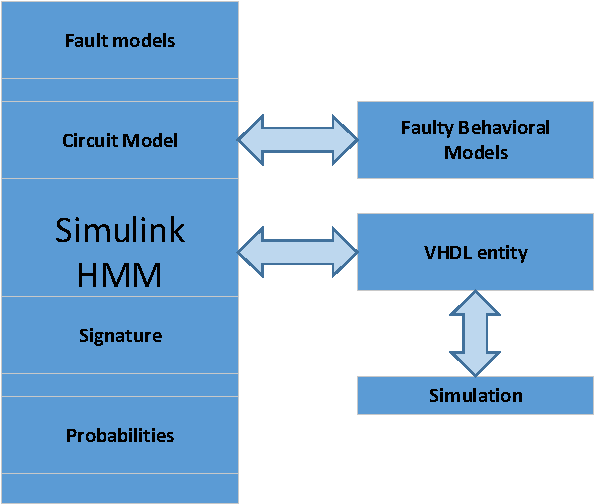
\includegraphics[scale=0.8]{Figures/simulink.pdf}
   \caption{Library creation}
\label{fig:lib}
\end{figure}




%\subsection{Emulation Environment and Framework}
%\subsection{Sequential Circuit Fault Injection Mechanism}
%\subsection{Sequential Circuit Test Generation}


%\section{Modeling in Sequential Circuit}
%\subsection{Soft-Error Modeling and Analysis in Sequential Circuit}
%
%
%To analyze the faulty behavior of the sequential circuit by using Markov Chain theory is quite obvious choice. Markov chain analysis provide the steady state behavior of the sequential circuit. By using MC analysis we will able to find the number of clock cycles the sequential circuit produce the faulty output.
%
%As mentioned in the section related work, single error rate can be categorized into three different categories a)  circuit level b) gate level and c) architectural level.  Our work is focused on the architectural level by emulating the fault at circuit level. 




%Most of the real-time application of the electronic systems are sequential in nature, e.g., random access memories. A typical sequential circuit comprises of combinational logic and flip-flop as shown in Figure.   Inputs of the combinational logic, output of the combinational logic, and inputs and outputs of the flip-flop. There is a temporal correlations between the input signal and the state signal. The state signals are uniquely identified as the function of the input signal and the previous state signal. Due to this; sequential circuit error propagation from the error site, e.g., a bit flip in a flip-flop to the output can observe after several clock cycles. This temporal relationship force to use the more dynamic models than the models availble for the combinational circuits. The sequential circuits models can evolve with the time instances.
%
%We will make our faulty model from the real-time radiation experiment. We will start our analysis by analysing the faulty values. Let us consider the example of the counter as shown in Figure 1 fault free and Figure 2 faulty where output is stuck at 1 .  
%
%
%We will start our analysis by error probability matrix associated with the circuit and the probability that the erros comes in any part of the circuit (Combinational or flip-flop) produce an error at the output. 





%\section{Markov Chain Analysis for Faulty Behaviour Model}
%
%   
%
%
%
%
%$NS^{original}$ $=$  $\delta^{o}$ $=$ $(\delta^{o}_{1},\delta^{o}_{2},\delta^{o}_{3},...,\delta^{o}_{m})$
%
%
%$NS^{faulty}$ $=$  $\delta^{f}$ $=$ $(\delta^{f}_{1},\delta^{f}_{2},\delta^{f}_{3},...,\delta^{f}_{m})$
%
%
%$\delta^{o}$ $=$ Fault-Free circuit output values
%
%$\delta^{f}$ $=$ Faulty circuit output values
%
%$m$ $=$ Number of output variables
%
%From there I can construct my signature vector:
%
%
%$\epsilon_{signature}$ $=$ $\delta^{o}$  $-$ $\delta^{f}$
%
%
%Now, the main goal for the soft error analysis for sequential circuits is to find the transistion probabilities between the signatures from the signature vector $\epsilon_{signature}$ and from there to determine the faulty behaviour of the sequential circuits when soft-error occurs. 
%
%\subsection{SER Measurement in Sequential Circuits}
%
%\subsection{Modeling with Probabilistic Calculation Methods}

%\subsection{Modeling of Sequential Circuit with Markovian-Chain Analysis}



%The fault injection platform proposes for this project emulates SEUs, more specifically single-bit upsets (SBUs) within the configuration memory of SRAM-based FPGAs. We will study the effects of SEU on sequential circuits, and introduce a  framework for analyzing and detecting them. We will do the modeling and analysis of sequential circuits susceptibility to soft errors. Accurate sequential SEU estimation requires capturing the mechanism of error propagation and masking at both combinational and sequential levels. The challenging task for the sequential circuits under SEUs: the difference between sequential and combinational circuits from the context of ATPG and single stuck-at fault model. In this project, we will concentrate on sequential synchronous circuits. The problem we will face and encounter that the controllability of auxiliary inputs and observability of secondary outputs for the sequential circuits.  We will study and implement a technique which eases sequential circuits testing and ATPG by making controllability and observability much simple.
%
%\subsection{Fault Injection}
%
%We need to examine the behavior of a design under faults. For fault injection there are two strategies: (a) \textit{Software based fault injection}, and (b) \textit{FPGA based fault injection}. 
%
%\begin{itemize}
%
%\item Two methods will develop for software based fault injection. First, the source HDL code is modified to allow fault injection. Second, the simulation tool is used to force the error injection during simulation. 
%\item For FPGA-based simulation, we will use single error mitigation core from Xilinx~\cite{xilinx}. The idea is to integrate this core with our system to generate a modified bitstreams to emulate the occurrence of errors. We will use this strategy.
%\end{itemize}





%%\section{Research Axis 3: Radiation Bombardment}
%This part of the project is a neutron-induced Single Event Effect test in a commercial FPGA from Xilinx. The primary objective is to investigate the radiation effects reliability for the critical application. We will implement the sequential circuit and data acquisition system. The results we want to achieve to drive signatures for the sequential circuits. Our focus is on the analyzing the impact of multiple errors in state flip-flops, during the cycles following the cycle when faults occur. The following milestones we want to achieve from radiation bombardment experiment.
%
%\begin{itemize}
%\item Modeling of SEU, MBU and analyzing their effect on logic circuits.
%\item Evaluation of changes in error rates due to SEUs in sequential circuits.
%\item Compute the error probability, and signatures from bit-upsets can vary for different outputs and different circuits. 
%\item Evaluation of the impact of multiple flip-flop upsets in sequential circuits.
%\item Determining the outputs that are most susceptible to errors due to faults in logic.
%\item Determining the parts of the circuit (gates or gate clusters) that have the largest impact on circuit error probability.
%\item Estimation of lower and upper bounds of circuit susceptibility to transient.
%\end{itemize} 
%%
%\section{Research Axis 3: High-level Modelling}
%
%To model and analyze the sequential circuit susceptibility to soft errors, we need to used the approximate methods, e.g.,
%\begin{itemize}
%
%\item Binary Decision Diagram and Algebraic decision diagram.
%\item Markov-chain analysis based error rate estimation, which can provide steady-state Single-Error rate estimates following a hit. 
%\item A  Monte Carlo for SEU Analysis of Sequential Circuits based on the probability of the bit-flips and estimates the states outputs and signatures.
%
%\end{itemize}
%\subsection{Simulator}
%
%We also have a plan to develop a simulator with the help of \textit{isoneo}. The simulator is based on the Matlab / Simulink models. The simulator takes the input a parameterization file corresponding to the operational architecture of the system. This file is generated from the configurator; it is in XML format.
%From this configuration, the simulator initially initializes a model of the system failure tree.
%This model is then exploited dynamically during the simulation phase to evaluate the level of reliability of the system and its components. The simulator executes the simulation model with the constraints and concludes a level of safety for each equipment and the global system.

%\section{Optional: Fault Mitigation}
%Fault-mitigation can be achieved in two ways: preventing faults from happening and
%recovering after their occurrence. Fault preventing is achieved by using hardened components and/or shielding. But fault preventative is not a viable solution in terms of a project cost. More complex fault-mitigation methodologies can be implemented at the architectural level. We need to develop some fault-mitigation strategies like triple module redundancy with  dynamic reconfiguration of the hardware~\cite{jacobs2012reconfigurable} and/or something like the work presented in 
%%Jacobs \emph{et al.}~\cite{jacobs2012reconfigurable} and Alderighi \emph{et al.}~\cite{violante} promote the use of SRAM-FPGAs for reconfigurable fault-tolerant space applications.
%~\cite{jacobs2012reconfigurable} used fault tolerance framework (RFT) that enables system designers to dynamically adjust a system's level of redundancy and fault mitigation based on the varying radiation incurred at different orbital positions. Notably, the reconfigurable fault tolerance framework in~\cite{jacobs2012reconfigurable} is based on an upset rate modeling tool that used to capture time-varying radiation effects in a given orbit.


\section{Project Plan}


\textbf{Summary}

\textbf{Phase  01:} The emulation platform will be the starting point of research. We will use the SEUs for the configuration memory upsets. Selection of a suitable benchmark, which is probably ITC'99~\cite{ITC}used for the testing purpose and signature generation.

\textbf{Phase  02:} Evaluate the radiation based experimental setup results for signature under the neutron radiation at Triumf.


\textbf{Phase 03:} Implement that above mentioned methodology and high-level model for soft-error of sequential circuits.

%\section{Timetable}
%The development of the tasks identified in Chapter~\ref{sec:approach}, and the most important milestones of this project are presented in Figure~\ref{timetable}.
%In our intentions, the design of a time predictable computer architecture, the development of novel timing analysis techniques, and the FPGA prototypes implementation will unfold as a series of sequential tasks with relatively small interleaving. Dependability and real-time requirements, on the other hand, should be kept in mind throughout the whole advancement of the project.

\begin{figure}[h]
\centering
\begin{tikzpicture}
\begin{ganttchart}[
x unit=0.36cm,
y unit title=1.0cm,
y unit chart=1.5cm,
%vgrid,
hgrid,
inline,
]{1}{48}
\gantttitle{Research Project}{48} \\
\gantttitle{2016}{12} \gantttitle{2017}{12} \gantttitle{2018}{12} \gantttitle{2019}{12}\\



\ganttbar[bar height=.4]{Literature Review and Comp .Exam}{6}{24}\\
%\ganttmilestone[]{Comp. Exam}{20}\\
%\ganttmilestone[]{AHS}{6}
%\ganttmilestone[]{TODAES}{12}\\
\ganttbar[bar height=.4]{Emulation Platform for Seq. ckt}{6}{35} \\
\ganttbar[bar height=.4]{Radiation Experiment}{13}{24} \\
\ganttbar[bar height=.4]{Modelling and Analysis}{25}{42} \\
%\ganttmilestone[]{TAAS}{30}\\
%\ganttbar[bar height=.4]{Novel Timing analysis techniques}{22}{38} \\
%\ganttmilestone[]{DAC}{36}\\
%\ganttbar[bar height=.4]{FPGA Implementation}{27}{38} \\
%\ganttmilestone[]{TRETS}{40}\\
\ganttbar[bar height=.4]{Tech. Demo.}{35}{42} \\
%\ganttmilestone[]{IAC}{44}\\
\ganttbar[bar height=.4]{Thesis Writing}{35}{46}
%\ganttmilestone[]{Thesis}{44}\\
%\ganttbar[bar height=.4]{The \emph{PolyOrbite} Project}{1}{44} 

%\ganttlink{elem0}{elem1}
%\ganttlink{elem0}{elem2}
%\ganttlink{elem0}{elem3}

%\ganttlink{elem3}{elem4}

%\ganttlink{elem5}{elem6}
%\ganttlink{elem5}{elem7}

%\ganttlink{elem7}{elem8}
\end{ganttchart}
\end{tikzpicture}
\caption{Timetable.}
\label{timetable}
\end{figure}









